\documentclass{article}
\usepackage{tikz}
\usepackage{pgfplots}
\pgfplotsset{compat=1.16}

\begin{document}

\begin{figure}[h]
    \centering
    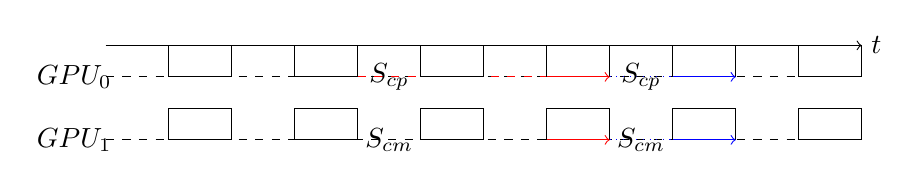
\begin{tikzpicture}[scale=0.8]
        % Draw the timeline
        \draw[->] (0,0) -- (12,0) node[right] {$t$};
        
        % Draw the horizontal lines for each GPU
        \draw[dashed] (0,-0.5) -- (12,-0.5);
        \draw[dashed] (0,-1.5) -- (12,-1.5);
        
        % Draw the GPU labels
        \node at (-0.5,-0.5) {$GPU_0$};
        \node at (-0.5,-1.5) {$GPU_1$};
        
        % Draw the synchronization lines
        \draw[red,dashed] (4,-0.5) -- (7,-0.5);
        \draw[blue,dotted] (8,-0.5) -- (9,-0.5);
        \draw[blue,dotted] (8,-1.5) -- (9,-1.5);
        
        % Draw the GPU kernels
        \foreach \x/\y in {1/-0.5, 3/-0.5, 5/-0.5, 7/-0.5, 9/-0.5, 11/-0.5} {
            \draw (\x,\y) rectangle ++(1,0.5);
        }
        \foreach \x/\y in {1/-1.5, 3/-1.5, 5/-1.5, 7/-1.5, 9/-1.5, 11/-1.5} {
            \draw (\x,\y) rectangle ++(1,0.5);
        }
        
        % Draw the synchronization labels
        \node at (4.5,-0.5) {$S_{cp}$};
        \node at (4.5,-1.5) {$S_{cm}$};
        \node at (8.5,-0.5) {$S_{cp}$};
        \node at (8.5,-1.5) {$S_{cm}$};
        
        % Draw the arrows indicating data dependency
        \draw[->,red] (7,-0.5) -- (8,-0.5);
        \draw[->,red] (7,-1.5) -- (8,-1.5);
        \draw[->,blue] (9,-0.5) -- (10,-0.5);
        \draw[->,blue] (9,-1.5) -- (10,-1.5);
    \end{tikzpicture}
    \caption{Two types of synchronization: inter-rank synchronization (red dashed line) and intra-rank/inter-stream synchronization (blue dotted line). For simplicity, we assume two GPUs and two streams ($S_{cp}$ and $S_{cm}$, for compute and communication respectively) per GPU, while CPU op calls are omitted in the plot. GPU kernels are represented by rectangles, and arrows indicate the data dependency between compute and communication kernels.}
    \label{fig:synchronization}
\end{figure}

\end{document}